\documentclass[onecolumn, draftclsnofoot,10pt, compsoc]{IEEEtran}
\usepackage{graphicx}
\usepackage{url}
\usepackage{setspace}

\usepackage{geometry}
\geometry{textheight=9.5in, textwidth=7in}

% 1. Fill in these details
\def \CapstoneTeamName{		The Cleverly Named Team}
\def \CapstoneTeamNumber{		12}
\def \GroupMemberOne{			Quanah Green}
\def \GroupMemberTwo{			Alex Ruef}
\def \GroupMemberThree{			Ethan Takla}
\def \CapstoneProjectName{		Remote Seed Identification}
\def \CapstoneSponsorCompany{	Crop and Soil Science Department, OSU}
\def \CapstoneSponsorPerson{		Dan Curry}

% 2. Uncomment the appropriate line below so that the document type works
\def \DocType{		%Problem Statement
				Requirements Document
				%Technology Review
				%Design Document
				%Progress Report
				}
			
\newcommand{\NameSigPair}[1]{\par
\makebox[2.75in][r]{#1} \hfil 	\makebox[3.25in]{\makebox[2.25in]{\hrulefill} \hfill		\makebox[.75in]{\hrulefill}}
\par\vspace{-12pt} \textit{\tiny\noindent
\makebox[2.75in]{} \hfil		\makebox[3.25in]{\makebox[2.25in][r]{Signature} \hfill	\makebox[.75in][r]{Date}}}}
% 3. If the document is not to be signed, uncomment the RENEWcommand below
\renewcommand{\NameSigPair}[1]{#1}

%%%%%%%%%%%%%%%%%%%%%%%%%%%%%%%%%%%%%%%
\begin{document}
\begin{titlepage}
    \pagenumbering{gobble}
    \begin{singlespace}
    	%\includegraphics[height=4cm]{coe_v_spot1}
        \hfill 
        % 4. If you have a logo, use this includegraphics command to put it on the coversheet.
        %\includegraphics[height=4cm]{CompanyLogo}   
        \par\vspace{.2in}
        \centering
        \scshape{
            \huge CS Capstone \DocType \par
            {\large\today}\par
            \vspace{.5in}
            \textbf{\Huge\CapstoneProjectName}\par
            \vfill
            {\large Prepared for}\par
            \Huge \CapstoneSponsorCompany\par
            \vspace{5pt}
            {\Large\NameSigPair{\CapstoneSponsorPerson}\par}
            {\large Prepared by }\par
            Group\CapstoneTeamNumber\par
            % 5. comment out the line below this one if you do not wish to name your team
            %\CapstoneTeamName\par 
            \vspace{5pt}
            {\Large
                \NameSigPair{\GroupMemberOne}\par
                \NameSigPair{\GroupMemberTwo}\par
                \NameSigPair{\GroupMemberThree}\par
            }
            \vspace{20pt}
        }
        \begin{abstract}
		abstract stuff

        \end{abstract}     
    \end{singlespace}
\end{titlepage}
\newpage
\pagenumbering{arabic}
\tableofcontents
% 7. uncomment this (if applicable). Consider adding a page break.
%\listoffigures
%\listoftables
\clearpage

\section{Introduction}
\subsection{Purpose}
In this document we outline the important qualities of the finished Remote Seed Certification project.
Don't really know what else to say here.

\subsection{Scope}
We will produce software that can process images containing seeds.
The processing will output information on the type of seeds and the quality (cleanliness) of the seeds.

\subsection{Definitions}
An important constraint on this project is that the users will send seeds in groups of 2500.
This will be called a sample.

\section{Overall Description}
\subsection{Product Perspective}
This project will be put in as a replacement to a part of the seed cleaning process.
Instead of sending the seed samples to a lab users will send images of the seeds to our processor.
Users will interface with our seed identification algorithm through a phone/tablet app.
Interface should be designed so that any non-technical person can learn to use in less than 1 hour
The app will then connect with our central processor over the internet.
After the processor has done its work the result will be stored in a database and sent back
to the user via email.

\subsection{Product Functions}
This project has 3 major components.
We need a phone/tablet app that can take pictures and send them to a Jetson TX2 processor.
On the Jetson processor will be an algorithm that can determine what seeds are in the picture and quality of the seeds.
The output of the algorithm will need to be saved in a database and sent to the user who sent the sample.

The app will need to be able to access the phones cameras and take pictures or pull from the users pictures.
Will we need rig to help take better pictures?
Will there need to be a rig to place the seeds in?
The app will then connect remotely to our Jetson processor and send the image.
Does the app need to be able to recieve processed image data or just send to users email?

Algorithm will use machine learning to decide what is in the images.
Can we deliver 2,500 seeds over 5 images?
Is this a design decision?
Stretch goal 2,500 seeds in one image.

Output will be in a pdf.
What will output look like?
what exact information needs to be conveyed?
Do we need to give information on each individual seed?
We will have a database to store this information and use it to improve learning algorithm.

\subsection{User Characteristics}
Users have wide range of education level.
Can't assume any level of technical prowess.
App should be "easily" used by anyone who has used a smart phone before. %define easily

\subsection{Constraints}
We are given a Jetson TX2 processor to use as the central processor.
The power of the Jetson will directly impact the processing time and the format of the input images.
Ask Dan about reliability requirements.

\subsection{Assumptions and Dependencies}
We rely heavily on the quality of images that phones and tablets can produce.

\section{Specific requirements}
\subsection{External interfaces}
\subsection{OpenCV}
Open Source Computer Vision Library will be used to implement our image processing and machine learning algorithm.
It will recieve image input from our app and it will output data on the quality and types of seeds.

\subsection{Functions}
This system shall open a connection to allow users to send images.
Validate that users are sending actual images.
Can we check the images for quality?
Jetson will then recieve image input.
Jetson will run our algorithm to determine seed type and quality in the image.
output will be stored in database.
PDF is then generated and sent back to the user.

\subsection{Performance Requirements}
Samples from users can be placed into a first in first out queue.
This will allow many users to send samples to our processor.
No clue how long it will take but the users will have to wait.

\subsection{Database Requirements}
Need more fine details on output of image processing.

\subsection{Standards Compliance}
Should ask Dan if he has any sample output from the seed lab.

\subsection{Reliability}
How reliable to we need to be and how can we insure that?

\subsection{Availability}
Probably only really needs to be up during the day.
Can be down at need to recover/restart.

\subsection{Security}
Mostly need to protect the Jetson.
validate incoming images to make sure they are images and don't contain malicious code.
Database is pretty safe since it is only accessed by Jetson.

\subsection{Maintainability}
Should make an attempt but its going to be hard being new to the technology.

\subsection{Portability}
App can be designed to be ported to IOS.
Image processing algorithm will probably be dependent on the Jetson.

\subsection{Objects}
May need objects to represent images and seeds.

\subsection{Features}
Would phone/tablet camera fit in here?

\section{Gantt Chart}
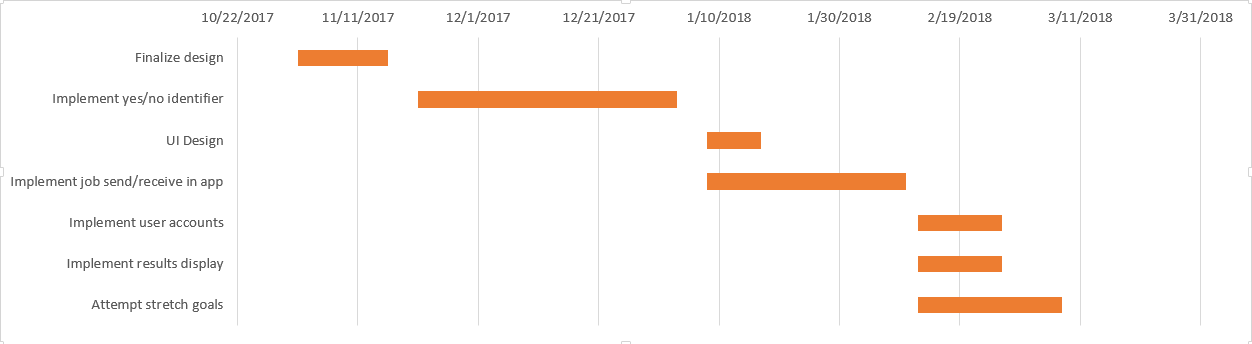
\includegraphics{gantt_chart.png}

\end{document}